\documentclass[table]{beamer}
\usepackage[utf8]{inputenc}
\usepackage[brazilian]{babel}
\usepackage{amsmath}
\usepackage{graphicx}
\usepackage{hyperref}
\usepackage{ragged2e}   
\usepackage{epstopdf}
\usepackage{multirow}
\usepackage{minted}
\usepackage{booktabs}

\setbeamertemplate{sidebar right}{}
\setbeamertemplate{footline}{%
\hfill\usebeamertemplate***{navigation symbols}
\hspace{1cm}\insertframenumber{}/\inserttotalframenumber}

\addtobeamertemplate{block begin}{}{\justifying}  %new code

\setbeamertemplate{footline}
{
  \leavevmode%
  \hbox{%
  \begin{beamercolorbox}[wd=.333333\paperwidth,ht=2.25ex,dp=1ex,center]{author in head/foot}%
    \usebeamerfont{author in head/foot}\insertsection
  \end{beamercolorbox}%
  \begin{beamercolorbox}[wd=.333333\paperwidth,ht=2.25ex,dp=1ex,center]{title in head/foot}%
    \usebeamerfont{title in head/foot}\insertsubsection
  \end{beamercolorbox}%
  \begin{beamercolorbox}[wd=.333333\paperwidth,ht=2.25ex,dp=1ex,right]{date in head/foot}%
    \usebeamerfont{date in head/foot}\insertshortdate{}\hspace*{2em}
    \insertframenumber{} / \inserttotalframenumber\hspace*{2ex} 
  \end{beamercolorbox}}%
  \vskip0pt%
}

\begin{document}

\begin{frame}
   \frametitle{Compiladores}
   \large
   \begin{center}
      O Processo de Varredura e Expressões Regulares 
   \end{center}
   \scriptsize
   \begin{center}
      João Marcelo Uchôa de Alencar \\
      joao.marcelo@ufc.br \\
      UFC-Quixadá
   \end{center}
\end{frame}

\begin{frame}
   \tableofcontents
\end{frame}

\begin{frame}
   \frametitle{Introdução}
   \begin{block}{Marcas ou \textit{tokens}}
   Sequência de caracteres que representam uma unidade de informação do programa fonte.
   \end{block}
   \begin{itemize}
      \item Palavras-chave;
      \item identificadores;
      \item símbolos especiais.
   \end{itemize}
   \begin{block}{Reconhecimento de Padrões}
   Expressões Regulares e Autômatos.
   \end{block}
\end{frame}

\section{O Processo de Varredura}
\begin{frame}
   \frametitle{O Processo de Varredura}
   \begin{columns}
      \begin{column}{0.5\textwidth}
         \begin{block}{Processo de Varredura}
	 Ler caracteres do código-fonte e organizá-los em unidades lógicas para outras fases do compilador.
	 \end{block}
      \end{column}
      \begin{column}{0.5\textwidth}
         
\includegraphics[width=\linewidth,height=\textheight,keepaspectratio]{figuras/varrer.png}
      \end{column}
   \end{columns}
\end{frame}

\begin{frame}[fragile]
   \frametitle{Marcas}
   \begin{minted}{c}
typedef enum 
   {IF, THEN, ELSE, PLUS, MINUS, NUM, ID, ...}
   TokenType;
   \end{minted}
   \begin{itemize}
      \item A marca IF tem como \textbf{lexema} ou valor, na maioria das linguagens, a cadeia \textit{if};
      \item palavras reservadas tem um único lexema;
      \item identificadores podem ter diversos lexemas;
      \item números tem como lexemas sua representação em cadeias, porém outros \textbf{atributos}, como o próprio valor númerico, podem ser armazenados no \textit{token};
      \item o \textit{token} ou marca final é a coleção de todos seus atributos.
   \end{itemize}
\end{frame}

\begin{frame}[fragile]
   \frametitle{Registro de Marcas}
   \begin{columns}
      \begin{column}{0.5\textwidth}
         \begin{minted}{c}
typedef struct {
   TokenType tokenval;
   char *stringval;
   int numval;
 }
	 \end{minted}
      \end{column}
      \begin{column}{0.5\textwidth}
         \begin{minted}{c}
typedef struct {
   TokenType tokenval;
   union {
      char *stringval;
      int numval;
   } attribute;
} TokenRecord;
	 \end{minted}
      \end{column}
   \end{columns}

   \begin{block}{Metodologia}
   Uma solução comum é o sistema de varredura retornar apenas o valor da marca e colocar os outros atributos em variáveis que possam ser acessadas por outras partes do compilador.
   \end{block}
\end{frame}

\begin{frame}[fragile]
   \frametitle{Interface com Analisador Sintático}
   \begin{minted}{c}
TokenType getToken(void);
   \end{minted}
   \begin{itemize}
      \item A varredura está sob controle do analisador sintático;
      \item em outras palavras, a varredura é invocada, não tem o controle do processo.
   \end{itemize}
\end{frame}

\section{Expressões Regulares}
\begin{frame}
   \frametitle{Expressões Regulares}
   \begin{columns}
      \begin{column}{0.5\textwidth}
         \begin{block}{Padrões}
            \begin{itemize}
               \item Uma expressão regular $r$ é completamente definida pelo conjunto de cadeias de caracteres com as quais ela casa;
	       \item linguagem gerada;
	       \item alfabeto $\Sigma$;
	       \item metacaracateres ou metasímbolos.
            \end{itemize}
        \end{block}
      \end{column}
      \begin{column}{0.5\textwidth}
         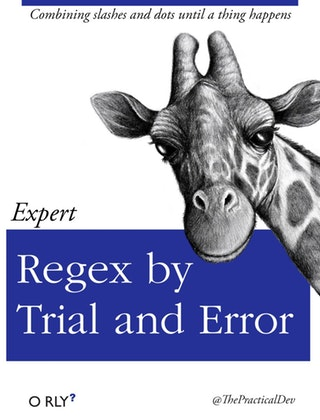
\includegraphics[width=\linewidth,height=\textheight,keepaspectratio]{figuras/trialanderror.jpg}
      \end{column}
   \end{columns}
\end{frame}

\begin{frame}
   \frametitle{Definição de Expressões Regulares}
   \begin{block}{Expressões Regulares Básicas}
      \begin{itemize}
         \item Dado um caractere \textit{a} de $\Sigma$, $L(a) = {a}$;
	 \item cadeia vazia: $\varepsilon$, $L(\varepsilon) = {\varepsilon}$;
	 \item conjunto vazio: $\Phi$, $L(\Phi) = \{ \}$. 
      \end{itemize}
   \end{block}
   \begin{block}{Operações de Expressões Regulares}
      \begin{itemize}
         \item Escolha entre alternativas: $|$;
	 \item concatenação;
	 \item repetição ou \textit{fecho}: *.
      \end{itemize}
   \end{block}
\end{frame}

\begin{frame}
   \frametitle{Definição de Expressões Regulares}
   \begin{block}{Escolha Entre Alternativas}
      \begin{itemize}
         \item Se $r$ e $s$ são ERs, então $r|s$ é uma ER;
	 \item casa com qualquer cadeia que case com $r$ \textbf{ou} $s$;
	 \item $L(r|s)=L(r) \cup L(s)$.
      \end{itemize}
   \end{block}
   \begin{block}{Concatenação}
      \begin{itemize}
         \item Se $r$ e $s$ são ERs, então $rs$ é uma ER;
	 \item casa cadeias que sejam concatenação de duas cadeias, desde que a primeira case com  $r$ e a segunda $s$;
	 \item $L(rs)=L(r)L(s)$.
      \end{itemize}
   \end{block}
\end{frame}

\begin{frame}
   \frametitle{Definição de Expressões Regulares}
   \begin{block}{Repetição}
      \begin{itemize}
         \item Se $r$ é uma ER, então $r^{*}$ é uma ER;
	 \item $r^{*}$ casa com qualquer concatenação finita de cadeias de caracteres, desde que cada cadeia case com $r$;
	 \item $L(r^{*})=L(r)^{*}$.
      \end{itemize}
   \end{block}
   \begin{block}{Precedência de Operações e Parênteses}
      \begin{itemize}
         \item $a|b^{*}$ significa $(a|b)^{*}$ ou $a|(b^{*})$?
	 \item $*$ tem maior precedência, seguido da concatenação e por último $|$;
	 \item os parênteses servem para alterar a ordem da precedência.
      \end{itemize}
   \end{block}
\end{frame}

\begin{frame}[fragile]
   \frametitle{Nomes ou Abreviaturas para ERs}
   Representar sequências de um ou mais dígitos:
   \begin{minted}{bash}
(0|1|2|3|4|5|6|7|8|9) (0|1|2|3|4|5|6|7|8|9)*
   \end{minted}
   ERs que aparecem com frequência podem ser abreviadas:
   \begin{minted}{bash}
digito digito*, onde:
digito = 0|1|2|3|4|5|6|7|8|9
   \end{minted}
\end{frame}

\begin{frame}
   \frametitle{Definição de Expressões Regulares}
   \begin{block}{Uma \textbf{expressão regular} é uma das seguintes:}
      \begin{enumerate}
         \item Uma expressão regular \textbf{básica}, composta por um único caractere \textbf{a}, onde $a$ pertence a um alfabeto $\Sigma$ de caracteres legais; o metacaractere $\varepsilon$; ou o metacaractere $\Phi$.
	 \item Uma expressão da forma $r|s$, onde $r$ e $s$ são expressões regulares. Nesse caso, $L(r|s) = L(r) \cup L(s)$.
	 \item Uma expressão da forma $rs$, onde $r$ e $s$ são expressões regulares. Nesse caso, $L(rs) = L(r)L(s)$.
	 \item Uma expressão da forma $r^{*}$, onde $r$ é uma expressão regular. Nesse caso, $L(r^{*}) = L(r)^{*}$.
	 \item Uma expressão da forma $(r)$, onde $r$ é uma expressão regular. Nesse caso, $L((r))=L(r)$. Assim parênteses não modificam a linguagem. Eles são utilizados apenas para ajudar a precedência de operadores.
      \end{enumerate}
   \end{block}
\end{frame}

\begin{frame}
   \frametitle{Exemplos de Expressões Regulares}
   \begin{itemize}
      \item $(a|c)^{*}b(a|c)^{*}$
      \item $(a|c)^{*}|(a|c)^{*}b(a|c)^{*}$
      \item Cadeias em $\Sigma = \{a,b\}$ compostas por um único $b$ rodeadas pelo mesmo número de $a$'s
      \item Cadeias em $\Sigma = \{a,b,c\}$ sem $b$'s consecutivos 
      \item $((b|c)^{*}a(b|c)^{*}a)^{*}(b|c)^{*}$
   \end{itemize}
\end{frame}

\begin{frame}
   \frametitle{Extensões de Expressões Regulares}
   \begin{block}{Uma ou Mais Repetições}
      \begin{itemize}
         \item Semelhante ao $*$;
	 \item \textit{uma} ou mais repetições em vez de zero ou mais repetições;
	 \item símbolo $+$.
      \end{itemize}
   \end{block}
   \begin{block}{Qualquer Caractere}
      \begin{itemize}
         \item Representar qualquer caractere do alfabeto;
	 \item o símbolo $.$ (ponto) é uma abreviatura para esse caso.
      \end{itemize}
   \end{block}
   \begin{block}{Intervalo de Caracteres}
      \begin{itemize}
         \item $a|b|...|z$ para letras e $0|1|...|9$ para números;
	 \item $[a-z]$ e $[0-9]$ desempenham o mesmo papel.
      \end{itemize}
   \end{block}
\end{frame}

\begin{frame}
   \frametitle{Extensões de Expressões Regulares}
   \begin{block}{Qualquer Caractere Fora de Um Dado Conjunto}
      \begin{itemize}
         \item O uso do circunflexo elimina qualquer caractere de um conjunto;
	 \item $[^\wedge abc]$.
      \end{itemize}
   \end{block}
   \begin{block}{Subexpressões Opcionais}
      \begin{itemize}
         \item Expressões que ocorrem uma vez ou nenhuma;
	 \item basta seguir a expressão com $?$.
      \end{itemize}
   \end{block}
\end{frame}

\begin{frame}[fragile]
   \frametitle{Expressões Regulares para Marcas}
   \begin{block}{Números}
      \begin{minted}{bash}
nat = [0-9]+
signedNat = (+|-)? nat
number = signedNat("." nat)?(E signedNat)?
      \end{minted}
   \end{block}
   \begin{block}{Palavras Reservadas e Identificadores}
      \begin{minted}{bash}
reservadas = if | while | do | ...

letra = [a-zA-Z]
digito = [0-9]
identificador = letra(letra | digito)*
      \end{minted}
   \end{block}
\end{frame}

\begin{frame}[fragile]
   \frametitle{Expressões Regulares para Marcas}
   \begin{block}{Comentários}
      \begin{itemize}
         \item Comentários de uma linha são simples;
	 \item comentários de várias linhas, estilo C, resultam em ERs complexas;
	 \item o desenvolvedor de compiladores acaba tratando de maneira \textit{ad hoc}.
      \end{itemize}
   \end{block}
\end{frame}

\begin{frame}[fragile]
   \frametitle{Expressões Regulares para Marcas}
   \begin{block}{Ambigüidade}
      \begin{itemize}
         \item Quando uma cadeia pode ser um identificador ou palavra-chave, a última prevalece;
	 \item \textbf{princípio da subcadeia mais longa}: a cadeia mais longa de caracteres que poderia constituir uma única marca deve representar a próxima marca;
	 \item \textit{whileYouWereSleeping} é um identificador, não o começo de um bloco \textit{while};
	 \item \textbf{delimitadores}: caracteres que fixam um fim para a subcadeia mais longa:
	 \begin{itemize}
	    \item operadores;
	    \item espaços em branco;
	    \item ponto-e-vírgula.
	 \end{itemize}
      \end{itemize}
   \end{block}
\end{frame}

\begin{frame}
   \frametitle{OFF-TOPIC: grep e awk}
   \begin{itemize}
      \item \textbf{grep} (exercício 2.3): ferramenta que analisa um fluxo de linhas (arquivos) e retorna quais elementos do fluxo casam com determinada ER;
      \item \textbf{awk}: linguagem de programação completa com foco na manipulação de cadeia de caracteres.
   \end{itemize}
\end{frame}

\section{Autômatos Finitos}
\begin{frame}
   \frametitle{Autômatos Finitos}
   \begin{columns}
      \begin{column}{0.5\textwidth}
         \begin{block}{Máquina de Reconhecimento}
         Autômatos finitos podem ser utilizados para descrever o processo de reconhecimento de padrões em cadeias de entrada.
	 \end{block}
      \end{column}
      \begin{column}{0.5\textwidth}
         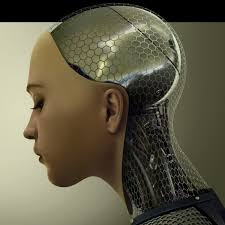
\includegraphics[width=\linewidth,height=\textheight,keepaspectratio]{figuras/automato.jpeg}
      \end{column}
   \end{columns}
\end{frame}

\begin{frame}[fragile]
   \frametitle{Autômatos Finitos}
   \begin{minted}{bash}
identificador = letra(letra|digito)*
   \end{minted}
   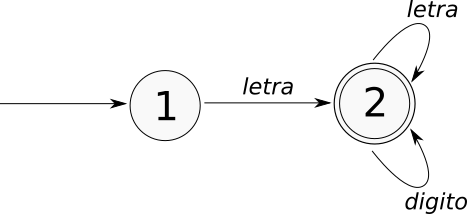
\includegraphics[width=\linewidth,height=\textheight,keepaspectratio]{figuras/automatofinitoidentificadores.png}
\end{frame}

\begin{frame}
   \frametitle{Autômatos Finitos}
   \begin{block}{Definição}
   Um \textbf{DFA} (autômato finito determinístico) $M$ é composto por:
      \begin{itemize}
         \item Um alfabeto $\Sigma$;
	 \item um conjunto de estados $S$;
	 \item uma função de transição $T:S x \Sigma \to S$;
         \item um conjunto de estados de aceitação $A \subset S$.
      \end{itemize}
   A linguagem aceita por $M$, denotada como $L(M)$, é definida como o conjunto de cadeias de caracteres $c_{1}c_{2}...c_{n}$ no qual cada $c_{i} \in \Sigma$ é tal que existem estados $s_{1}=T(s_{0}, c_{1}), s_{2}=T(s_{1}, c_{2}), ... , s_{n}=T(s_{n-1}, c_{n})$ em que cada $s_{n}$ é um elemento de $A$ (ou seja, um estado de aceitação).  
   \end{block}
\end{frame}

\begin{frame}
   \frametitle{Autômatos Finitos}
   \begin{block}{Algumas simplificações:}
      \begin{enumerate}
         \item Utilizamos números para os estados no diagrama do identificador, mas a definição não restringe o conjunto de estados a números;
	 \item para evitar inúmeras transições, podemos usar abreviaturas de classes de caracteres se todos os membros tenham o mesmo estado origem e destino;
	 \item a definição exige que exista uma transição para cada par $(s_{i}, c_{i})$, porém podemos não representar aquelas que não levam a estados de aceitação.
      \end{enumerate}
   \end{block}
\end{frame}

\begin{frame}[fragile]
   \frametitle{Autômatos Finitos}
   \begin{block}{Exemplos}
      \begin{enumerate}
         \item O conjunto de cadeias de caracteres que contém exatamente um $b$;
	 \item o conjunto de cadeias de caracteres que contém no máximo um $b$;
	 \item comentários da linguagem C;
	 \item constantes númericas em notação científica: 
      \end{enumerate}
   \end{block}
   \begin{minted}{bash}
   digito = [0-9]
   nat = digito+
   signedNat = (+|-)? nat
   numero = signedNat("." nat)?(E signedNat)?
   \end{minted}
\end{frame}

\begin{frame}
   \frametitle{Verificação à Frente}
   \begin{block}{Programa de varredura que implementa o Autômato:}
      \begin{itemize}
         \item Ação de transição: mover caractere da entrada para o lexema da marca;
	 \item ação de aceitação: retornar a marca, lexema e outros atributos;
	 \item ação de erro: voltar atrás na entrada ou gerar uma marca de erro.
      \end{itemize}
   \end{block}
   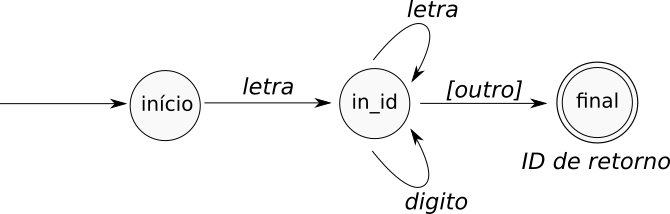
\includegraphics[width=\linewidth,height=\textheight,keepaspectratio]{figuras/automatodelimitador.png}
\end{frame}

\begin{frame}
   \frametitle{Marcas e Autômatos}
   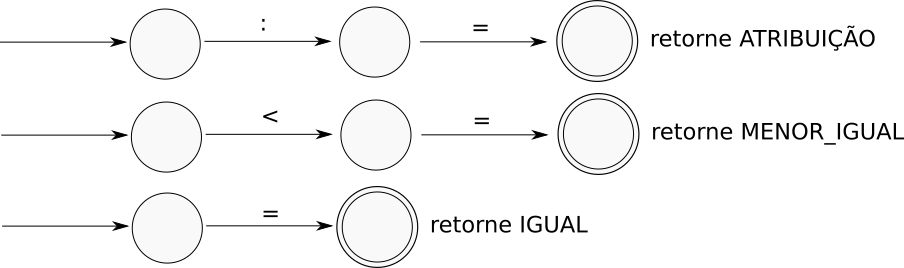
\includegraphics[width=\linewidth,height=\textheight,keepaspectratio]{figuras/menorigual00.png}<1>
   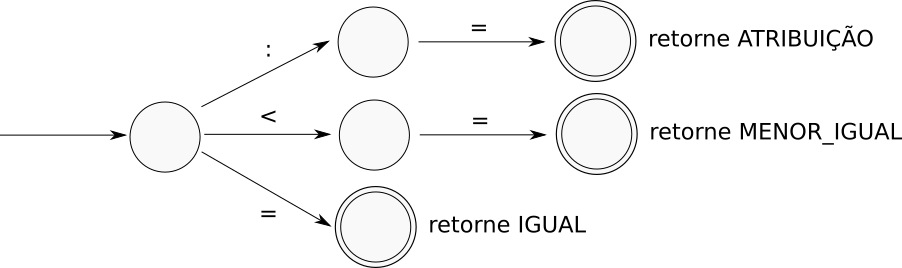
\includegraphics[width=\linewidth,height=\textheight,keepaspectratio]{figuras/menorigual01.png}<2>
   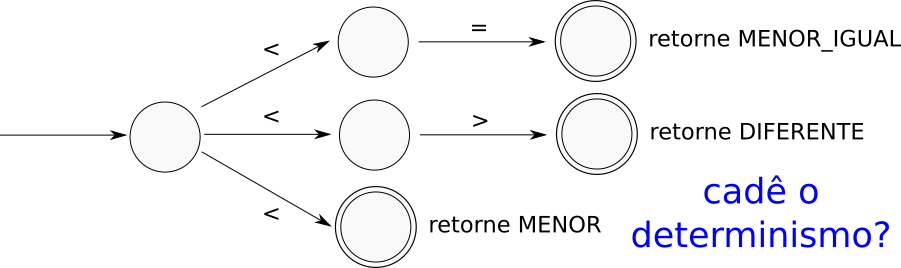
\includegraphics[width=\linewidth,height=\textheight,keepaspectratio]{figuras/menorigual02.png}<3>
   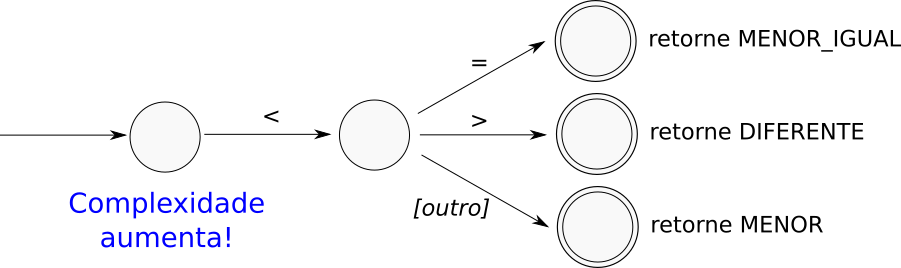
\includegraphics[width=\linewidth,height=\textheight,keepaspectratio]{figuras/menorigual03.png}<4>
\end{frame}

\begin{frame}
   \frametitle{Autômato Finito Não Determinístico}
   \begin{block}{Motivação}
      \begin{itemize}
         \item Expandir a definição de DFA para incluir o caso de mais de uma transição de um estado para um caractere em particular;
	 \item desenvolver algoritmo para transformar os novos autômatos em DFAs;
	 \item \textbf{$\varepsilon$-transição} é uma transição que pode ocorrer sem consultar a cadeia de entrada.
      \end{itemize}
   \end{block}
\end{frame}

\begin{frame}
   \frametitle{Marcas e Autômatos}
   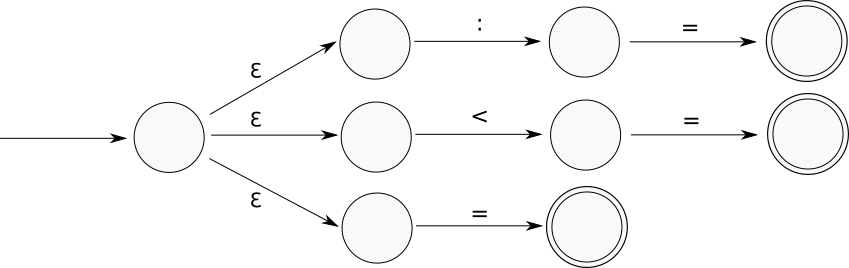
\includegraphics[width=\linewidth,height=\textheight,keepaspectratio]{figuras/menorigual04.png}
\end{frame}

\begin{frame}
   \frametitle{Autômato Finito Não Determinístico}
   \begin{block}{Definição}
   Um \textbf{NFA} (autômato finito não determinístico) é composto por:
       \begin{itemize}
          \item Um alfabeto $\Sigma$;
	  \item um conjunto de estados $S$;
	  \item uma função de transição $T:Sx\Sigma \cup \{\varepsilon\} \to \varphi(S)$;
	  \item um estado inicial $s_{0} \in S$;
	  \item um conjunto de estados de aceitação $A \subset S$.
       \end{itemize}
   A linguagem aceita por $M$, denotada como $L(M)$, é definida como o conjunto de cadeias de caracteres $c_{1}c_{2}...c_{n}$ em que cada $c_{i}$ de $\Sigma \cup \{\varepsilon\}$ para qual existam estados  $s_{1}$ em $T(s_{0},c_{1}), s_{2}$ em $T(s_{1}, c_{2})$, ... , $s_{n}$ em $T(s_{n-1}, c_{n})$, em que $s_{n}$ seja elemento de $A$.   
   \end{block}
\end{frame}

\begin{frame}
   \frametitle{Autômato Finito Não Determinístico}
   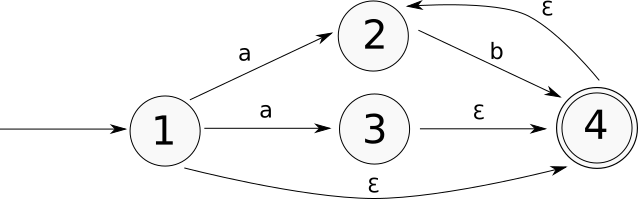
\includegraphics[width=\linewidth,height=\textheight,keepaspectratio]{figuras/exemplonfa.png}
   \\
   \\
   \centering
   Qual é a expressão regular?
\end{frame}

\begin{frame}[fragile]
   \frametitle{Implementação em Código de Autômatos Finitos}
   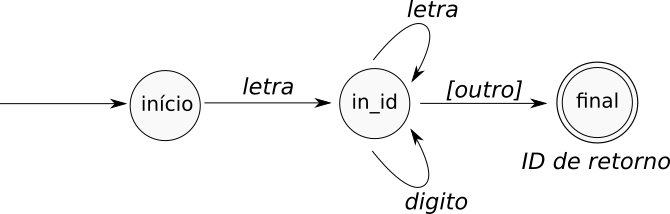
\includegraphics[width=\linewidth,height=\textheight,keepaspectratio]{figuras/automatodelimitador.png}
   \footnotesize
   \begin{minted}{pascal}
   {início - estado 1}
   if proximo caractere letra then
      avance entrada;
      {in_id - estado 2}
      while proximo caractere letra ou digito do
         avance entrada; {permanece no estado 2}
      end while;
      {passa para o estado final - 3 - sem avancar na entrada}
      aceitacao;
   else
      {erro ou outros casos}
   end if;
   \end{minted}
\end{frame}

\begin{frame}
   \frametitle{Implementação em Código de Autômatos Finitos}
   \begin{itemize}
      \item O estado é armazenado de forma implícita, de acordo com a posição do código na execução;
      \item é um código \textit{ad hoc}, ou seja, foi criado a partir da observação das transições do autômato, mas sem obedecer a uma metodologia sistemática;
      \item para três estados, o código está coeso. Mas para uma quantidade maior de estados, a complexidade aumenta de forma considerável.
   \end{itemize}
\end{frame}

\begin{frame}[fragile]
   \frametitle{Implementação em Código de Autômatos Finitos}
   \scriptsize
   \begin{minted}{pascal}
{estado 1}
if proximo caractere igual a / then
  avance entrada; {estado 2}
  if proximo caractere igual a * then
    avance entrada; {estado 3}
    fim := false;
    while not fim do
      while proximo caractere diferente de * do
        avance entrada;
      end while;
      avance entrada; {estado 4}
      while proximo caractere for * do
        avance entrada;
      end while;
      if proximo caractere igual a / then
        fim := true;
      end if;
      avance entrada;
    end while;
    aceitacao; {estado 5}
  else {outro processamento}  
  end if;
else {outro processamento}  
end if;
   \end{minted}
\end{frame}

\begin{frame}[fragile]
   \frametitle{Usando \textit{case/switch} para Organizar o Caos}
   \begin{itemize}
      \item Uma variável para manter o estado atual;
      \item um laço, com um primeiro \textit{case} testando o estado e outro o caractere;
   \end{itemize}
   \footnotesize
   \begin{minted}{pascal}
estado := 1; {inicio}
while estado = 1 ou estado = 2 do
  case estado of
  1: case caractere de entrada of
     letra: avance entrada;
            estado := 2;
     else estado := ... {erro ou outro};
     end case;
  2: case caractere de entrada of
     letra, digito: avance entrada;
                    estado := 2; {desnecessario}
     else estado := 3;
     end case;
  end case;
end while;
if estado = 3 then aceitacao else erro;
   \end{minted}
\end{frame}

\begin{frame}[fragile]
   \frametitle{Usando \textit{case/switch} para por Ordem no Caos}
   \scriptsize
   \begin{minted}{pascal}
estado := 1; {inicio}
while estado = 1, 2, 3 ou 4 do
  case estado of
  1: case caractere de entrada of
     / : avance entrada;
         estado := 2;
     end case;
  2: case caractere de entrada of
     * : avance entrada;
         estado := 3;
     else estado := ... {erro ou outro};
     end case;
  3: case caractere de entrada of
     * : avance entrada;
         estado := 4;
     else avance entrada {continua no estado 3}
     end case;
  4: case caractere de entrada of
     / : avance entrada;
         estado := 5;
     * : avance entrada; {continha no estado 4}
     else avance entrada;
          estado := 3;
  end case;
end while;
if estado = 5 then aceitacao else erro;
   \end{minted}
\end{frame}

\begin{frame}
   \frametitle{Tabela de Transição}
   \centering
   \begin{table}
      \begin{tabular}{c|c}
       & Caracteres no alfabeto $c$ \\
      \hline 
      Estados $s$ & Estados que representam transições $T(s,c)$ \\
   \end{tabular}
   \end{table}

   \begin{table}
      \begin{tabular}{|c|c|c|c|c|}
      \hline
      \textit{caractere de entrada} & \textit{letra} & \textit{digito} & \textit{outro} & \textit{Aceitação} \\
      \textbf{estado} & & & &\\
      \hline
      \textbf{1} & 2 & & & não \\
      \textbf{2} & 2 & 2 & [3] & não \\
      \textbf{3} &   &   & & sim  \\
      \hline
      \end{tabular}
   \end{table}
\end{frame}

\begin{frame}[fragile]
   \frametitle{Algoritmo para Autômatos com Tabela de Transição}
   \begin{minted}{pascal}
estado := 1;
ch := proximo caractere;
while not Aceita[estado] and not erro(estado) do
  novoestado := T[estado, ch].
  if Avance[estado, ch] then ch := proximo caractere;
  estado := novo estado;
end while
if Aceita[estado] then aceitacao;
   \end{minted}
\end{frame}

\begin{frame}
   \frametitle{Observações}
   \begin{itemize}
      \item Algoritmos dirigidos por tabela são simples, mas consomem muita memória;
      \item um algoritmo para NFA teria que armazenar vários fluxos de derivações, só retornando sucesso caso uma delas termine em aceitação;
      \item portanto, algoritmos que trabalham diretamente com NFAs são ineficientes. Melhor transformar o NFA em DFA e aplicar os algoritmos apresentados. 
   \end{itemize}
\end{frame}

\section{ER para DFA}
\begin{frame}
   \frametitle{A Estrada de uma ER para um DFA}
   \begin{block}{O caminho mais simples...}
   O algoritmo mais simples para traduzir uma ER para um DFA usa um NFA intermediário.
   \end{block}
   \vspace{1.0cm}
   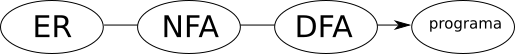
\includegraphics[width=\linewidth,height=\textheight,keepaspectratio]{figuras/ernfadfa.png}
\end{frame}

\begin{frame}
   \frametitle{De uma ER para um NFA}
   \begin{block}{Construção de Thompson}
   Usamos transições $\varepsilon$ para juntar máquinas de cada pedaço de uma expressão regular e formar uma máquina correspondente à expressão toda.
   \end{block}
\end{frame}

\begin{frame}
   \frametitle{Expressões Regulares Básicas}
   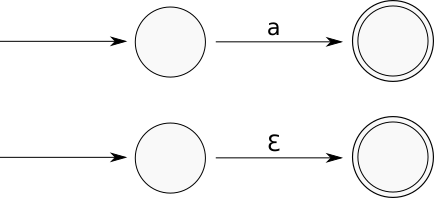
\includegraphics[width=\linewidth,height=\textheight,keepaspectratio]{figuras/erbasica.png}
\end{frame}

\begin{frame}
   \frametitle{Concatenação}
   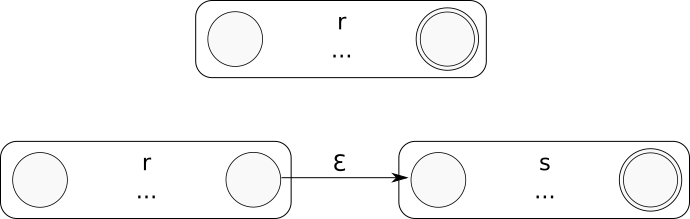
\includegraphics[width=\linewidth,height=\textheight,keepaspectratio]{figuras/concatenacao.png}
\end{frame}

\begin{frame}
   \frametitle{Escolha entre Alternativas}
   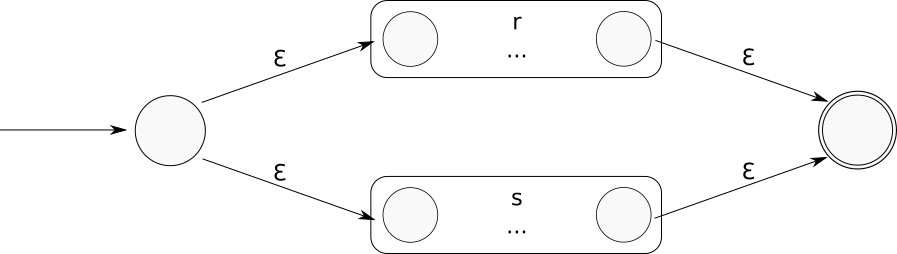
\includegraphics[width=\linewidth,height=\textheight,keepaspectratio]{figuras/alternativas.png}
\end{frame}

\begin{frame}
   \frametitle{Repetição}
   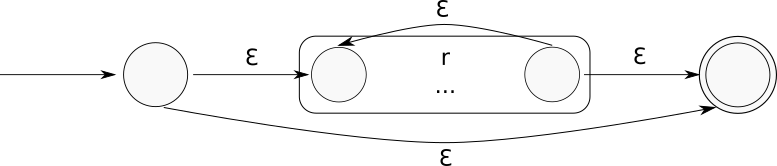
\includegraphics[width=\linewidth,height=\textheight,keepaspectratio]{figuras/repeticao.png}
\end{frame}

\begin{frame}
   \frametitle{Exemplos para Construção de Thompson}
   \begin{block}{Criar um NFA para as ERs:}
      \begin{itemize}
         \item $ab|a$;
         \item $letra(letra|digito)^{*}$.
      \end{itemize}
   \end{block}
\end{frame}

\begin{frame}
   \frametitle{De um NFA para um DFA}
   \begin{block}{Construção de Subconjuntos}
      \begin{itemize}
         \item Precisamos eliminar transições $\varepsilon$ e múltiplas;
	 \item um $\varepsilon$-\textbf{fecho} é o conjunto de todos os estados atingíveis por $\varepsilon$-transições a partir de um estado ou estados;
	 \item a eliminação de transições múltiplas a partir de um estado para um caractere requer o acompanhamento do conjunto de estados atingíveis pelo casamento de um único caractere.
      \end{itemize}
   \end{block}
\end{frame}

\begin{frame}
   \frametitle{De um NFA para um DFA}
   \begin{block}{O $\varepsilon$-fecho de um Conjunto de Estados}
   O $\varepsilon$-fecho de um único estado $s$ é o conjunto de estados atingíveis por uma série de zero ou mais $\varepsilon$-transições, denominado $\bar{s}$. O $\varepsilon$-fecho de um conjunto de estados $S$ é dado por: $\bar{S} = \bigcup\limits_{s \in S}\bar{s}$. 
   \end{block}
   \begin{block}{Construção de Subconjuntos}
   \footnotesize
   Para construir um DFA $\bar{M}$ partir de um NFA $M$:
      \begin{enumerate}
         \item Definimos $S^{'} = \O$ como o conjunto de estados de $\bar{M}$;
         \item adicionamos a $S^{'}$ o estado inicial de $\Bar{M}$ como o $\varepsilon$-fecho do estado inicial de $M$;
	 \item enquanto novos estados ainda forem criados:
	 \begin{enumerate}
	    \item dado um caractere $a$ do alfabeto defina $S^{'}_{a} = \{t|$ para algum $s \in S$ existe uma transição de $s$ para $t$ em $a\}$. 
	    \item defina $\bar{S^{'}_{a}}$ e o adicione a $S^{'}$.
	    \item defina a nova transição $S \xrightarrow{a} \bar{S^{'}_{a}}$ 
	 \end{enumerate}
	 \item todos os estados de $S^{'}$ que contenham um estado de aceitação de $M$ são de aceitação em $\bar{M}$.
      \end{enumerate}
   \end{block}
\end{frame}

\begin{frame}
   \frametitle{Exemplos para Construção de Subconjuntos}
   \begin{block}{Exemplos}
      \begin{itemize}
         \item $a^{*}$
	 \item $ab|a$
	 \item $letra(letra|digito)^{*}$
      \end{itemize}
   \end{block}
\end{frame}

\begin{frame}
   \frametitle{Minimização do Número de Estados de um DFA}
   \begin{block}{Algoritmo de Hopcroft}
      \begin{itemize}
         \item Dividir os estados do autômato original em dois conjuntos, aceitação e não aceitação;
	 \item analisar quais transições ocorrem para os próprios dois novos estados e entre eles, considerando cada caractere do alfabeto;
	 \item analisar, dentro de cada estado, quais transições distinguem os estados internos entre si;
	 \item repartir os estados caso haja distinção;
	 \item repetir o processo até não existir mais distinções.
      \end{itemize}
   \end{block}
\end{frame}

\section{Varredura para TINY}
\begin{frame}
   \frametitle{Marcas para a Linguagem TINY}
\begin{table}
   \begin{tabular}{c|c|c}
   \hline
   Palavras Reservadas & Símbolos Especiais & Outras\\
   \hline 
   if & + & \textit{número} \\
   then & - & (1 ou mais dígitos) \\
   else & * & \\
   end & / & \\
   repeat & = & \\
   until & $<$ & \textit{identificador}\\
   read & $($ & (1 ou mais letras)\\
   write & $)$ & \\
   & $;$ & \\
   & $:=$ & \\
   \hline
   \end{tabular}
   \begin{block}{Comentários} 
   Comentários são cercados por chaves $\{$...$\}$ e não pode ser aninhados.
   \end{block}
\end{table}
\end{frame}

\begin{frame}
   \frametitle{DFA para a Linguagem TINY}
   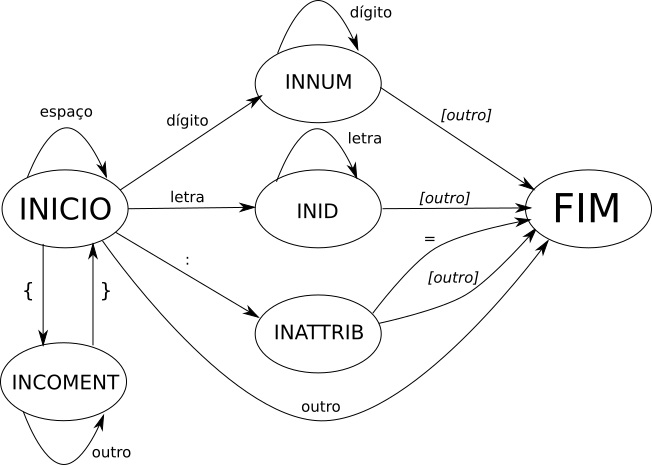
\includegraphics[width=\linewidth,height=\textheight,keepaspectratio]{figuras/tinydfa.png}
\end{frame}

\begin{frame}
   \frametitle{Discussão do Código}
   \begin{itemize}
      \item Arquivos \textbf{scan.h} e \textbf{scan.c} no Apêndice B do livro do Louden;
      \item o principal procedimento é \textsf{getToken}, consome caracteres de entrada e devolve a marca reconhecida de acordo com o DFA;
      \item utiliza a metodologia do \textit{case} aninhado, com um \textit{if-then-else} no lugar de um dos \textit{case} para melhorar a legibilidade;
      \item as marcas estão definidas no arquivo \textbf{globals.h};
      \item em TINY, o único atributo é o próprio \textit{lexema} (ver \textit{scan.h});
      \item variávels globais: \textit{source, listing} e \textit{lineno};
   \end{itemize}
\end{frame}

\begin{frame}
   \frametitle{Discussão do Código}
   \begin{block}{Funcionamento de getToken}
      \begin{itemize}
         \item A tabela \textbf{reservedWords} e o procedimento \textit{reservedLookup} verificam palavras reservadas;
	 \item uma variável de controle \textit{save} é utilizada para indicar se um caractere será adicionado a \textbf{tokenString};
	 \item \textbf{getNextChar} vai adicionando caracteres a partir de \textbf{linebuf}.
      \end{itemize}
   \end{block}
\end{frame}

\begin{frame}[fragile]
   \frametitle{Programa Exemplo na Linguagem TINY}
   \begin{minted}{pascal}
{
   Programa de exemplo na 
   linguagem TINY - computa o fatorial
}
read x; {entrada de um inteiro}
if 0 < x then { não calcula se x <= 0}
   fact := 1;
   repeat
      fact := fact * x;
      x := x - 1;
   until x = 0;
   write fact {saída do fatorial de x}
end
   \end{minted}
\end{frame}

\section{Lex}
\begin{frame}
   \frametitle{Uso do Lex para Gerar um Sistema de Varredura}
   \begin{itemize}
      \item Vamos repetir a criação de um analisador léxico, agora usando uma ferramenta que automatiza o processo: \textit{Lex};
      \item é um programa que recebe como entrada um arquivo contendo \textbf{expressões regulares} e \textbf{ações} associadas a cada expressão;
      \item é gerado um procedimento \textit{yylex}, implementação de um DFA.
   \end{itemize}
\end{frame}

\begin{frame}
   \frametitle{Convenções Lex para Expressões Regulares}
   \begin{itemize}
      \item Usar aspas para qualquer caractere que se deseje o casamento direto, seja metacaractere ou não;
      \item $* + ( ) | ?$ tem o significado já discutido;
      \item $[abxz]$ e  $[a-z]$ também são suportados;
      \item conjunto complementar: $[^\wedge0-9abc]$;
      \item dentro dos colchetes, a maioria dos metacaracteres perde seu \textit{status} especial;
      \item uso de chaves para nomear expressões regulares.
   \end{itemize}
\end{frame}

\begin{frame}[fragile]
   \frametitle{Convenções Lex para Expressões Regulares}
   \begin{minted}{bash}
("aa"|"bb")("a"|"b")*"c"?

nat [0-9]+
signedNad (+|-)? {nat}
   \end{minted}
\end{frame}

\begin{frame}[fragile]
   \frametitle{Formato de um Arquivo de Entrada Lex}
   \begin{block}{Composto por três partes:}
   Uma coleção de \textbf{definições}, uma coleção de \textbf{regras} e uma coleção de \textbf{rotina auxiliares}.
   \end{block}
   \begin{minted}{bash}
{definições}
%%
{regras}
%%
{rotinas auxiliares}
   \end{minted}
\end{frame}

\begin{frame}[fragile]
   \frametitle{Formato de um Arquivo de Entrada Lex}
   \begin{minted}{bash}
%{
/* programa Lex para adicionar números
   de linhas a linhas de um texto, e 
   imprimir o novo texto
*/
#include<stdio.h>
int lineno = 1;
%} 
line .*\n
%%
{line} { printf("%5d %s", lineno++, yytext); }
%% 
main()
{ yylex(); return 0;}
   \end{minted}
\end{frame}

\begin{frame}[fragile]
   \frametitle{Gerando o Programa}
   \begin{minted}{bash}
$ lex numeralinha.l 
$ gcc lex.yy.c -o numeralinha
$ ./numeralinha < numeralinha.l 
    1 %{
    2 /* programa Lex para adicionar números
    3    de linhas a linhas de um texto, e 
    4    imprimir o novo texto
    5 */
...
   \end{minted}
\end{frame}

\begin{frame}
   \frametitle{Explicando a Entrada Lex}
   \begin{itemize}
      \item O que está entre os delimitadores \%\{ e \%\} é inserido no código, sem alteração;
      \item em seguida definimos uma expressão regular com o nome \textit{line};
      \item após \%\%, temos a ação a ser tomada toda vez que a entrada casar com a expressão;
      \item \textbf{yytex} é o nome que Lex dá à cadeia que casa com a expressão;
      \item o código após o último \%\% é inserido ao final do código C gerado;
      \item \textbf{yylex} é o nome dado à função do DFA implementado.
   \end{itemize}
\end{frame}

\begin{frame}
   \frametitle{Convenções do Lex}
   \begin{itemize}
      \item Se um caractere ou cadeia de caracteres não casar com nenhuma expressão regular, Lex ecoará a entrada na saída;
      \item Lex sempre casa com a subcadeia mais longa;
      \item se a subcadeia mais longa casar com duas regras, Lex seleciona a primeira regra definida.
   \end{itemize}

   \begin{table}
      \begin{tabular}{c|c}
      \hline
      Nome & Significado \\
      \hline 
      lex.yy.c ou lexyy.c & Arquivo de Saída \\
      yylex & Função do DFA \\
      yytext & Cadeia que casa com a ER \\
      yyin & Entrada Lex \\
      yyout & Saída Lex \\
      input & Rotina de entrada \\
      ECHO & Ação Básica \\
      \hline
      \end{tabular}
   \end{table}
\end{frame}

\begin{frame}
   \frametitle{Finalizamos Varredura}
   Dúvidas?
\end{frame}

\end{document}

